\documentclass{patmorin}
\listfiles
\usepackage{amsthm,amsmath,graphicx,wrapfig}
\usepackage{pat}
%\usepackage{coffee4}
\usepackage[letterpaper]{hyperref}
\usepackage[dvipsnames]{color}
\definecolor{linkblue}{named}{Blue}
\hypersetup{colorlinks=true, linkcolor=linkblue,  anchorcolor=linkblue,
citecolor=linkblue, filecolor=linkblue, menucolor=linkblue, pagecolor=linkblue,
urlcolor=linkblue} \setlength{\parskip}{1ex}

\newcommand{\lstlabel}[1]{\label{lst:#1}}
\newcommand{\lstref}[1]{Listing~\ref{lst:#1}}
\newcommand{\Lstref}[1]{\lstref{#1}}

\usepackage{listings}
\usepackage{minted}
\usepackage{mdframed}
\surroundwithmdframed{minted}

\title{\MakeUppercase{Array Layouts for Comparison-Based Searching}}
\author{Paul-Virak Khuong and Pat Morin}


\begin{document}
\begin{titlepage}
\maketitle

\begin{abstract}
  This experimental work studies the best order in which to store $n$
  data items in an array, $A$, of length $n$ so that one can, for any
  query value, $x$, quickly find the smallest value in $A$ that is greater
  than or equal to $x$. In particular, we consider the important case
  where there are many such queries to the same array, $A$.  In addition
  to the obvious sorted-order we consider the Eytzinger (BFS) layout
  normally used for heaps, an implicit B-tree layout that generalizes
  the Eytzinger layout, and the van Emde Boas layout commonly used in
  the cache-oblivious algorithms literature.

  After extensive testing and tuning on a wide variety of modern hardware,
  we arrive at the conclusion that, for small values of $n$, sorted
  order, combined with a good implementation of binary search is best.
  For larger values of $n$, we arrive at the surprising conclusion that
  the Eytzinger layout is the fastest when executing a single sequence
  of queries.  The latter conclusion was unexpected and constradicts
  earlier experimental work by Brodal, Fagerberg, and Jakob (SODA~2003),
  who concluded that both the B-tree and van Emde Boas layouts were faster
  than the Eytzinger layout for large values of $n$.  The reason for this
  discrepancy is that, since 2003, processors have changed qualitatively.
\end{abstract}

\end{titlepage}

\section{Introduction}

A sorted array combined with binary search represents \emph{the} classic
data structure/query algorithm pair: theoretically optimal, fast in
practice, and discoverable by school children playing guessing games.
Although sorted arrays are \emph{static}---they don't support efficient
insertion or deletion---they still have many practical applications
involving bulk-processing of data, and even na\"{\i}ve implementations
of binary search execute searches several times faster than the most
popular dynamic data structures.\footnote{For example, Barba and Morin
\cite{bmXX} found that a naive implementation of binary search in a
sorted array was approximately three times faster than searching using
C++'s \texttt{stl::set} class.}

However, that sorted order is just one possible order that can be used to
store data in an array. Other layouts are also possible and---combined
with the right query algorithm---may allow for faster queries.
Other array layouts may be able to take advantage of (or be hurt less
by) modern processor features such as caches, instruction pipelining,
conditional moves, speculative execution, and prefetching.

In this experimental paper we consider four different memory layouts and
accompanying search algorithms.  All of these memory layouts store $n$
data items in a single array of length $n$, and their accompanying search
algorithm can find (say) the index of the largest value in the array that
is greater than or equal to $x$ for any value $x$.\footnote{In case $x$
is greater than any value in the array, the search algorithm returns
the index $n$.}

\begin{enumerate}
  \item \texttt{Sorted}:  This is the usual sorted layout, in which
  the data is stored in sorted order and searching is done using binary
  search.

  \item \texttt{Eytzinger}: In this layout, the data is viewed as being
  stored in a complete binary search tree.  The root of this tree is
  stored at $A[0]$, and the left and right children of the node stored
  at $A[i]$ are stored at $A[2i+1]$ and $A[2i+2]$, respectively.

  \item \texttt{Btree}: In this layout, the data is viewed as being stored
  in a complete $(b+1)$-ary tree, so that each node stores $b$ values.
  The parameter $b$ is chosen so that $b$ values fit neatly into a single
  cache line and the nodes of this tree mapped to array locations using
  a generalization of the Eytzinger mapping:  For $j\in \{0,\ldots,b\}$,
  the $j$th child of the node that starts at position $i$ is stored
  beginning at position $i(b+1)+(j+1)b$.

  \item \texttt{vEB}: In this, the \emph{van Emde Boas} layout, the data
  is viewed as being stored in a complete binary tree whose height is
  $h=\lceil\log (n+1)\rceil -1$. This tree is layed out recursively:  If
  $h=0$, then the single node of the tree is stored in $A[0]$.  Otherwise,
  the tree is split into a top-part of height $\lfloor h/2\rfloor$,
  which is recursively layed out starting at $A[0]$.  Attached to the
  leaves of this top tree are $2^{1+\lfloor{h/2\rfloor}}$ subtrees,
  which are recursively layed out, in left-to-right order, starting at
  array location $A[2^{1+\lfloor{h/2\rfloor}}-1]$.
\end{enumerate}


\subsection{Related Work}

Brodal, Fagerberg, and Jakob.


These guys look at array layouts of multidimensional arrays within programming languages:

\url{https://engineering.purdue.edu/~mithuna/pubs/ics99.pdf}


\subsection{Summary of Results}

Our findings, with respect to a single process executing repeated random
searches on a single array, $A$, are summarized as follows:

\begin{enumerate}
  \item For small values of $n$ (smaller than the L1 cache), branch-free
    implementations of search algorithms are considerably faster, by nearly
    a factor of two.
  
  \item For small values of $n$ (smaller than the L3 cache), a good
    branch-free implementation of binary search is unbeaten by any other
    strategy.  A branch-free implementation of the Eytzinger layout is a
    close second.
  
  \item For large values of $n$ (larger than the L3 cache), the branch-free
    implementation of binary search is among the worst of all algorithms,
    followed closely by the branch-free implementations of the Eytzinger
    algorithms.
  
  \item For large values of $n$ (larger than the L3 cache), the branchy
    implementations of search algorithms usually perform better than the
    branch-free implementations.  Branch prediction, even though it is
    incorrect and leads to a pipeline flush 50\% of the time triggers
    the memory subsystem to load a cache line that is correct 50\%
    of the time.  

  \item For large values of $n$, the fastest method is the Eytzinger layout
   combined with a branch-free search that uses explicit prefetching.
\end{enumerate}

\section{Processor Architecture Considerations}

In this section, we briefly review, at a very high level, the elements of
modern processor architecture that affect our findings.  For concreteness,
we will use numbers from a recent high-end desktop processor, the Intel
4790K \cite{S} with 4 8GB DDR3-1866 memory modules.

\subsection{CPU}

At the highest level, a computer system consists of a processor (CPU)
connected to a random access memory (RAM). On the Intel 4790K, the
CPU runs at frequency of 4GHz, or $4\times10^9$ cycles per second.
This CPU can execute roughly $4\times 10^{9}$ instructions per
second.\footnote{This is only a very rough approximation of the
truth; different instructions have different latencies and throughput
\cite{granlund.instruction}.}

\url{https://gmplib.org/~tege/x86-timing.pdf}


\subsection{RAM, Latency, and Transfer Rate}

The RAM, on ths system runs at 1866MHz, or roughly $1.866\times10^9$
cycles per second.

Transfer rate: This RAM module can transfer 8 bytes per cycle from RAM
to the CPU, for a (theoretical) peak transfer rate of 
$8\times 1.866\times10^9\approx 15$GB/s.

First-Word Latency: This RAM module has a \emph{first-word latency} of
approximately 10ns: From the time a processor issues a memory request
to that memory is available is approximately $10^{-8}$ seconds.

Observe that, if the CPU repeatedly reads 4 byte quantities from RAM,
then it receives $10^8$ of these per second, for a transfer rate of
$4\times 10^8=0.4$GB/s.  Note how far this is below this peak transfer
rate of 15GB/s.

In a similar vein, if the CPU is executing instructions that require
the contents of memory locations in RAM, and a subsequent instruction
can not begin before the previous instruction completes, then the CPU
will not execute more than $10^8$ instructions per second; it will waste
approximately 39/40 cycles waiting on data from RAM.

Cache-Line (8th-Word) Latency:  When the CPU reads a RAM address, the
RAM moves a 64 byte cache line into the CPU. From the time CPU issues
the access to the time the last word of the cache-line is available is
approximately 13.4ns.  If the processor repeatedly reads cache lines
from RAM, this results in a transfer rate of $64 / (13.4\times10^{-9})
\approx 4.8$GB/s.  Observe that this is still less than a third of the
RAM's peak transfer rate.

To actually achieve a transfer rate close to the theoretical peak transfer
rate, the CPU must issue memory read requests before previous requests
have finished. This will be important and is ultimately the reason that
the Eytzinger layout outperforms other layouts.

\subsection{Caches}

Since reading from RAM is a relatively slow operation, processors use
several levels of caches between the processor and the RAM.

The Intel 4790K has a 32KB L1 data cache (per core), a 256KB L2 cache
(per core), and an 8MB L3 cache (shared among 4 cores).  Each of these
cache levels is successively slower than the previous level, with L1 being
the fast and L3 being the slowest; but still much faster than RAM.

\subsection{The Prefetcher}

To help achieve peak memory throughput and avoid having the processor
stall while waiting on RAM, the CPU includes a prefetcher that analyzes
memory access patterns in an attempt to predict future memory accesses.
For instance, in simple code such as the following:

\begin{minted}{c++}
    long sum = 0;
    for (int i = 0; i < n; i++) 
        sum += a[i];
\end{minted}

The prefetcher is likely to detect that memory allocated to array
\mintinline{c++}{a} is being accessed sequentially.  The prefetcher will
then load blocks of \mintinline{c++}{a} into the cache hierarchy even
before they are accessed.  By the time the code actually needs the value
of \mintinline{c++}{a[i]} it will already be available in L1/L2/L3 cache.

Prefetchers on current hardware can detect simple access patterns
like the sequential pattern above.  More generally, they can often
detect arithmetic progressions of the form $a,a+k,a+2k,a+3k,\ldots$
and even interleaved arithmetic progressions such as $a, b, a+k, b+r,
a+2k,b+2r,a+3k,b+3r,\ldots$.  However, current technology does not go
much beyond this.

\subsection{Translation Lookaside Buffer}

As part of modern virtual memory systems, the processor has a
\emph{translation lookaside buffer (TLB)} that maps virtual memory
addresses (visible to processes) to physical memory addresses (addresses
of physical RAM).  Since a TLB is used for every memory access, it is very
fast, and not very large.  TLBs organizes memory into fixed-size pages.
A process that uses multiple pages of memory will sometimes access a
page that is not in the TLB. This is costly, and triggers the processor
to walk the \emph{page table} until it finds the appropriate page and
then it loads the entry for this page into the TLB.

The Intel 4790K has three data TLBs: The first contains 4 entries for
1GB pages, the second contains 32 entries for 2MB pages, and the third
contains 64 entries for 4KB pages.  In our experiments---which were done
on a dedicated system running few other processes---TLB misses were not
a significant factor until the array size exceeded 4GB.



\subsection{Pipelining, Branch-Prediction, and Predicated Instructions}

Executing an instruction on a processor takes several clock cycles, during
which the instruction is (1)~fetched, (2)~decoded, an (3)~effective
address is read (if necessary), and finally the instruction is
(4)~executed.  Since the entire process takes several cycles, this
arranged in a pipeline so that, for example, one instruction is being
executed while the next instruction is reading a memory address, while
the next instruction is being decoded, while the next instruction is
being fetched.

This all works well provided that the CPU knows which instruction to
fetch.  Where this breaks down is in code that contains \emph{conditional
jump} instructions. These instructions will possibly change the flow of
execution based on the result of some previous comparison.  In such cases,
the CPU does not know in advance whether the following instruction will
be the one immediately after the conditional jump or will be the target
of the conditional jump. The CPU has two options: 
\begin{enumerate}
  \item Wait until the condition that determines the output
   of the jump has been tested. In this case, the insruction pipeline
   is not being filled from the time the conditional jump instruction
   enters the pipleline until the the time the jump condition is tested.

  \item Predict whether the jump will occur or not and begin loading
  the instructions from the jump target, or immediately after the jump,
  respectively.  In this case, if the prediction is correct, then no
  time is wasted. If the prediction is incorrect, then once the jump
  condition is finally verified, all instructions placed in the pipeline
  after the conditional jump instruction have to be flushed.
\end{enumerate}

Most modern processors implement the second option and implement
some form of \emph{branch predictor} to obtain accurate predictions.
Branch predictors work well when the condition is highly predictable so
that, e.g., the conditional jump is almost never or almost always taken.

Most modern processors use some form of two-level adaptive predictor
\cite{yeh.patt.two-level} that can even handle second-order statistics,
such as conditional jumps that implement loops with a fixed number of
iterations. In this case, they can detect conditions such as ``this
conditional jump is taken $k$ times consecutively and then not taken
once.''  In standard benchmarks, representative of typical work-loads,
branch-predictor success rates above 90\% and even above 95\% are not
uncommon \cite{X}.

Another useful tool used to avoid branch misprediction (and branches
altogether) is the conditional move \mintinline{nasm}{cmov} family
of instructions.  Introduced into Intel architectures in 1995 with
the Pentium Pro line, these are instructions that move the contents of
one register to another (or to memory), but only if some condition is
satisfied. They do not change the flow of execution and therefore do
not interfere with the processor pipeline.

Conditional moves are a special case of \emph{predicated
instructions}---instructions that are only executed if some predicate
is true.  The Intel IA-64 and ARM CPU architectures include extensive
predicated instruction sets.

\section{The Layouts}

In this section, we provide an in-depth discussion the implementation
and performance of the four array layouts we tested.

\subsection{Sorted}

Searching a sorted array is an especially important special case. Every
major programming language and environment provides a sorting routine,
so a sorted array is usually just a function call away. Many language
also provide a matching binary search implementation.  In C++,
sorting is done with \mintinline{c++}{std::sort()} and binary
search is implemented in \mintinline{c++}{std::lower_bound()} and
\mintinline{c++}{std::upper_bound()}. 

The chromium browser code-base, for example, calls these
implementations of binary search from 135 different locations
in a wide variety of contexts, including cookie handling, GUI
layout, graphics and text rendering, video handling, and certificate
management.\footnote{\url{https://goo.gl/zpSdXo}}  This is the code-base
on which Google Chrome, which now boasts over 1 billion users \cite{X}, is
based. Improvements to \mintinline{c++}{std::lower_bound()}
and \mintinline{c++}{std::upper_bound()} could improve the user experience
of hundreds of millions of users.

\subsubsection{Na\"{\i}ve Binary Search}

The source code for na\"{\i}ve binary search is shown in
\lstref{nbs}. This code implements binary search the way it is typically
taught in introductory computer science courses.

\begin{listing}
\begin{minted}[linenos]{c++}
template<typename T, typename I>
I sorted_array<T,I>::branchy_search(T x) const {
    I lo = 0;
    I hi = n;
    while (lo < hi) {
        I m = (lo + hi) / 2;
        if (x < a[m]) {
            hi = m;
        } else if (x > a[m]) {
            lo = m+1;
        } else {
            return m;
        }
    }
    return hi;
}
\end{minted}
\caption{Source code for na\"{\i}ve binary search.}
\lstlabel{nbs}
\end{listing}

Let $C$ be the cache size (measured in data items) and $W$ is the
cache-line width (measured in data items).  Caching affects classic
binary search in two ways.

If $n> C/W$ is much larger than $C$ then, after a large number of
accesses, we expect to find the most frequently accessed values in the
cache.  These are the values at the top of the (implicit) binary search
tree implemented by binary search.  Since $n>C/W$, each of these values
will occupy their own cache line, so the cache only has room for $C/W$
of these.

Furthermore, once binary search has reduced the search range down to a
size less than or equal to $W$, the subarray that remains to be searched
will occupy at most one or two cache lines. Thus, on average, we expect
binary search to incur roughly $\log n -\log(C/W) - \log W + 1 = \log n -
\log C + 1$ cache misses.

Our test machine, the Intel 4790K, has 8192KB (8MB) of L3 cache and its
cache lines are 64 bytes wide.  With 4-byte data this gives the values
$W=16$ and $C=2048K=2^{21}$.
Therefore, once $n$ exceeds $2^{21}$, we expect a sharp increase in search
time, with each additional level of binary search incurring another
L3 cache miss and access to RAM.  When plotted with the $n$-axis on a
logarithmic scale, this shows up as an increase in slope at approximately
$n=2^{21}$.

\figref{sorted-i} shows the running time of $2\times 10^6$ searches
for values of $n$ ranging from 1 to $2^{27}$. As the preceding analysis
predicts, there is indeed a sharp increase in slope that occurs at around
$n=2^{21}$.  To give our results a grounding in reality, this graph
also shows the running-time of the \mintinline{c++}{stl::lower_bound()}
implementation---The C++ Standard Template Library implementation
of binary search.  Our na\"{\i}ve implementation and the
\mintinline{c++}{stl::lower_bound()} implementation perform nearly
identically.


\begin{figure}
   \centering{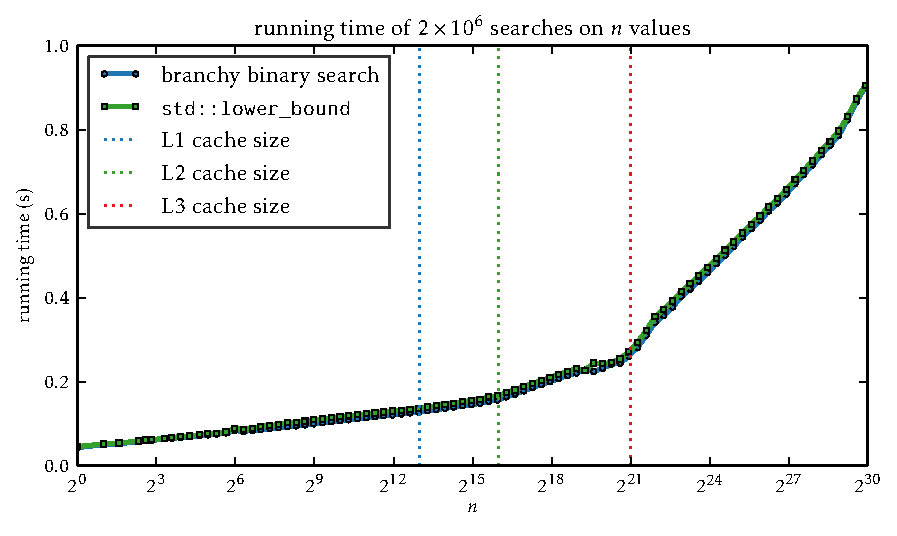
\includegraphics[width=.98\textwidth]{figs/sorted-i}}
   \caption{The running time of na\"{\i}ve binary search and \mintinline{c++}{stl::lower_bound()}.}
   \figlabel{sorted-i}
\end{figure}

If we consider only values of $n$ up to $2^{21}$, shown in
\figref{sorted-ii}, we see an additional change in slope at
$n=2^{16}$.  This is the same effect, but at the L2/L3 cache level; the
4790K has a 256KB L2 cache capable of storing $64K=2^{16}$ data items.
Each additional level of binary search beyond that point incurs an
additional L2 cache miss and access to L3 cache.

\begin{figure}
   \centering{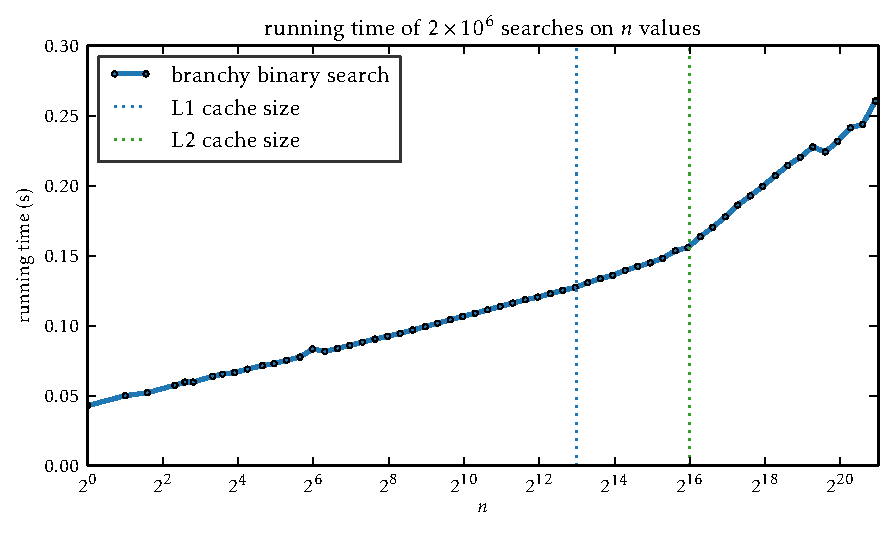
\includegraphics[width=.98\textwidth]{figs/sorted-ii}}
   \caption{The running time of na\"{\i}ve binary search when all data
    fits into L3 cache.}
   \figlabel{sorted-ii}
\end{figure}


\subsubsection{Branch-Free Binary Search}

Someone with experience in micro-optimizing code will see that, for
modern desktop processors, the code in \lstref{nbs} can be improved
substantially.  There are two problems with this code:

\begin{enumerate}

\item Inside the code is a three-way if statement whose execution path
is highly unpredictable. Each of the first two branches has a close to
$50\%$ chance of being executed.  The branch-predictor of a pipelined
processor is forced to guess which of these branches will occur and load
the instructions from this branch into the pipelline.  When it guesses
incorrectly (approximately 50\% of the time), the entire pipeline must be
flushed and the instructions for the other branch loaded.

\item The number of iterations of the outer loop is hard to predict. The
loop may terminate early (because \mintinline{c++}{x} was found). Even when
searching for a value \mintinline{c++}{x} that is not present, unless $n$ has
form $2^k-1$, the exact number of iterations is different for different
values of $x$.  This implies that the branch predictor will frequently
mispredict termination or non-termination of the loop, incurring the
cost of another pipeline flush.

\end{enumerate}

\Lstref{bfbs} shows an alternative implementation of binary search
that attempts to alleviate both problems described above.  In this
implementation, there is no early termination and, for a given array
length \mintinline{c++}{n}, the number of iterations is fixed (because the
value of \mintinline{c++}{n} always decreases by \mintinline{c++}{half}
during each iteration of the loop).  Therefore, when this method is
called repeatedly on the same array, a good branch-predictor will very
quickly learn the number of iterations of the \mintinline{c++}{while}
loop, and it will generate no further branch mispredictions.

\begin{listing}
\begin{minted}[linenos]{c++}
template<typename T, typename I>
I sorted_array<T,I>::_branchfree_search(T x) const {
    const T *base = a;
    I n = this->n;
    while (n > 1) {
        const I half = n / 2;
        base = (base[half] < x) ? &base[half] : base;
        n -= half;
    }
    return (*base < x) + base - a;
}
\end{minted}
\caption{Source code for branch-free binary search.}
\lstlabel{bfbs}
\end{listing}

In the interior of the \mintinline{c++}{while} loop, there is only
one piece of conditional code, which occurs in Line~7.  (For readers
unfamiliar with C's choice operator, this code is equivalent
to \mintinline{c++}{if (base[half] < x) base = &base[half]}.)
This line either reassigns the value of \mintinline{c++}{base} (if
\mintinline{c++}{base[half] < x}) or leaves it unchanged.  The compiler
implements this using a \emph{conditional move} (\mintinline{nasm}{cmov})
instruction so that there is no branching within the while loop.

The use of conditional move instructions to replace branching is
often a topic of heated debate (see, e.g., \cite{X}).  Conditional move
instructions tend to use more clock cycles than traditional instructions
and, in many cases, branch predictors can achieve prediction accuracies
exceeding 95\%, which makes it faster to use a conditional jump.  In this
particular instance, however, the branch predictor will be unable to make
predictions with accuracy exceeding 50\%, making a conditional move the
best choice.  The resulting assembly code, shown in \lstref{bfbs-asm} is
very lean.  The body of the \mintinline{c++}{while} loop is implemented
by Lines~8--15 with the conditional move at Line~12.


\begin{listing}
\begin{minted}[linenos]{nasm}
  .cfi_startproc
  movq    8(%rdi), %rdx       # move n into rdx
  movq    (%rdi), %r8         # move a into r8
  cmpq    $1, %rdx            # compare n and 1
  movq    %r8, %rax           # move base into rax
  jbe    .L2                  # quit if n <= 1
.L3:
  movq    %rdx, %rcx          # put n into rcx
  shrq    %rcx                # rcx = half = n/2
  leaq    (%rax,%rcx,4), %rdi # load &base[half] into rdi
  cmpl    %esi, (%rdi)        # compare x and base[half]
  cmovb   %rdi, %rax          # set base = &base[half] if x > base[half]
  subq    %rcx, %rdx          # n = n - half
  cmpq    $1, %rdx            # compare n and 1
  ja    .L3                   # keep going if n > 1
.L2:
  cmpl    %esi, (%rax)        # compare x to *base
  sbbq    %rdx, %rdx          # set dx to 00..00 or 11...11
  andl    $4, %edx            # set dx to 0 or 4 
  addq    %rdx, %rax          # add dx to base
  subq    %r8, %rax           # compute base - a (* 4)
  sarq    $2, %rax            # (divide by 4)
  ret
  .cfi_endproc
\end{minted}
\caption{Compiler-generated assembly code for branch-free binary search.}
\lstlabel{bfbs-asm}
\end{listing}

\Figref{sorted-iii} compares the performance of the na\"{\i}ve and
branch-free implementations of binary search for array sizes $n$
ranging from 1 to $2^{16}$.  As expected, the branch-free code is much
faster. Indeed, after accounting for the overhead of the testing harness,
the branch-free search is approximately twice as fast for $n=2^{16}$.

\begin{figure}
   \centering{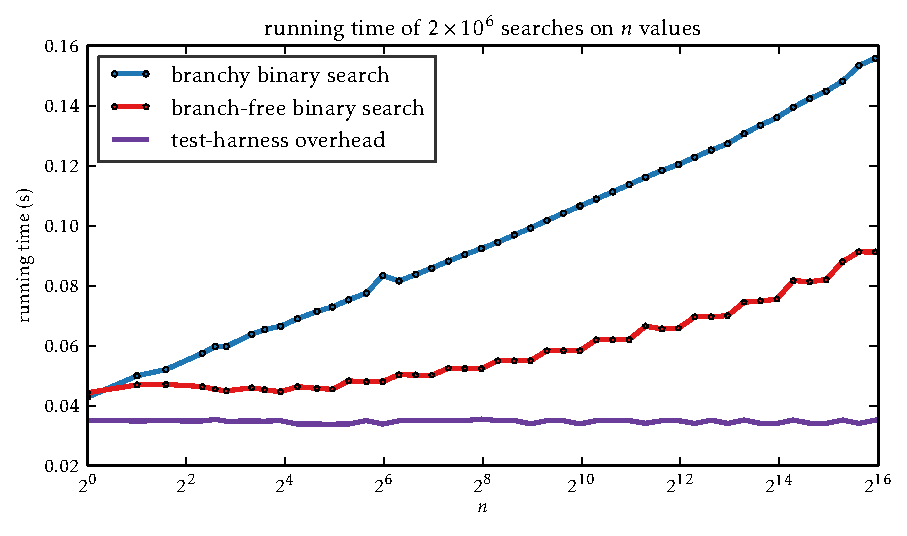
\includegraphics[width=.98\textwidth]{figs/sorted-iii}}
   \caption{The running times of na\"{\i}ve binary search versus
    branch-free binary search when all data
    fits into L3 cache.}
   \figlabel{sorted-iii}
\end{figure}

However, for larger values of $n$ (shown in \figref{sorted-iv}) the
situation changes.  For $n>2^{16}$, the gap begins to narrow until
slowly and for $n>2^{21}$ it narrows more quickly.  By the time time $n$
exceeds $2^{22}$, the branch-free code is slower and the gap between
the two continues to widen from this point onward.

\begin{figure}
   \centering{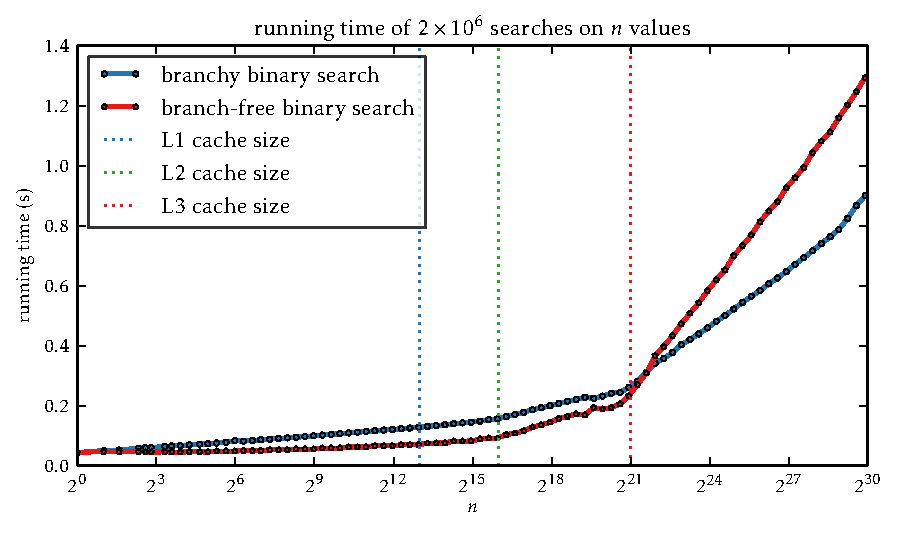
\includegraphics[width=.98\textwidth]{figs/sorted-iv}}
   \caption{The running times of na\"{\i}ve binary search versus
    branch-free binary search for large values of $n$.}
   \figlabel{sorted-iv}
\end{figure}

The reason for this change in relative performance was not immediately
obvious to us.  After some experimentation, we discovered it comes
from the interplay between branch prediction and the memory subsystem.
In the na\"{\i}ve code, the branch-predictor makes a guess at which branch
will be taken and is correct approximately half the time. An incorrrect
guess causes a costly pipeline flush.  However, a correct guess results
in the memory subsystem starting to load the array location needed during
the next iteration of the \mintinline{c++}{while} loop.

For small $n<2^{16}$, the entire array fits into L2 cache, and the costs
of pipeline flushes exceed any savings obtained by correct guesses.
However, for larger $n$, each correct guess by the branch-predictor
triggers an L2 (in the range $2^{16}<n<2^{21}$) or an L3 (for $n>2^{21}$)
cache miss sooner than it would otherwise.  The costs of these cache
misses are greater than the costs of the pipeline flushes, so eventually,
the branch-free code loses out to the na\"{\i}ve code.

Since this was not our initial explanation, and since it was not obvious
from the beginning, we gathered several pieces of evidence to support
or disprove this hypothesis.

\begin{enumerate}
\item Assembly-level profiling showed that, for large $n$, the
  branch-free code spends the vast majority of its time loading from
  memory (Line~11, of \lstref{bfbs-asm}).  This is because the register,
  \mintinline{nasm}{rdi},  containing the memory address to load is the
  target of a conditional move (Line~12).  This conditional move has not
  completed because it is still waiting on the results of the previous
  comparison, so the CPU stalls at this point.

\item Another possible explanation for our results was that the hardware
   prefetcher was, for some reason, better able to handle the na\"{\i}ve
   code than the branch-free code.  This seemed unlikely, since the memory
   access patterns for both version are quite similar, and probably too
   complicated for a hardware prefetcher to predict. Nevertheless, we
   ruled out this possibility by disabling the hardware prefetcher and
   running the tests again.\footnote{TODO: Add details of how to do this.
   We used the \mintinline{console}{wrmsr} command.}  The running-times
   of the code were unchanged by disabling prefetching.

\item We implemented a version of the branch-free code that adds explicit
   prefetching. At the top of the while loop, it
   prefetches array locations \mintinline{c++}{a[half/2]}
   and \mintinline{c++}{a[half+half/2]} using \texttt{gcc}'s
   \mintinline{c++}{__builtin_prefetch()} builtin, which translates into
   the x86 \mintinline{nasm}{prefetch0} instruction.  The performance of
   the resulting code, shown in \figref{sorted-v} is consistent with our
   hypothesis.  The code is nearly as fast as the branch-free code for
   small values of $n$, but tracks (and even improves) the performance
   of the na\"{\i}ve code for larger values of $n$.

\begin{figure}
   \centering{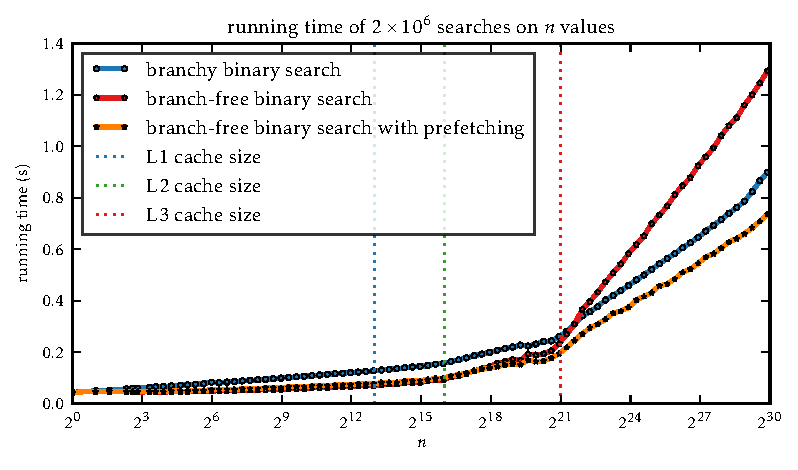
\includegraphics[width=.98\textwidth]{figs/sorted-v}}
   \caption{Branch-free binary search with explicit prefetching is competitive
    for small values of $n$ and a clear winner for large values of $n$.}
   \figlabel{sorted-v}
\end{figure}

\item We ran our code on Atom 330 processor that we had available.  This
   low-power processor does not do any form or speculative
   execution, including branch-prediction.  The result, which are
   shown in \figref{sorted-atom} are consistent with our hypothesis.
   The branch-free code is faster than the branchy code across the full
   range of values for $n$. The branch-free code with explicit prefetching
   matches the performance of the branch-free code for small $n$, and
   then outperforms it for larger $n$.
\end{enumerate}

From our study of binary search, we conclude the following lesson about
the (very important) case where one is searching in a sorted array:

\begin{lesson}
  For searching in a sorted array, the fastest method uses branch-free
  code with explicit prefetching.  This is true both on modern pipelined
  processors that use branch prediction and on traditional sequential
  processors.
\end{lesson}

We finish our discussion of binary search by pointing out one lesser-known
caveat:  If $n$ is large and very close to a power of 2, then all three
variants of binary search discussed here will have poor cache utilization.
This is caused by cache-line aliasing and is hinted at by Brodal \etal\
\cite{X} and discussed in detail by the first author \cite{X}.


TODO: Discuss the problem with array sizes that are (nearly) powers of two.

\subsection{Eytzinger}

\subsubsection{The Na\"{\i}ve Eytzinger Code}

The na\"{\i}ve implemntation of search in an Eytzinger array is nearly
as simple as that of binary search.

\begin{listing}
\begin{minted}[linenos]{c++}
template<typename T, typename I, bool aligned>
I eytzinger_array<T,I,aligned>::_branchy_search(T x) const {
	I j = n;
	I i = 0;
	while (i < n) {
		if (x < a[i]) {
			j = i;
			i = 2*i + 1;
		} else if (x > a[i]) {
			i = 2*i + 2;
		} else {
			return i;
		}
	}
	return j;
}

\end{minted}
\end{listing}



\subsubsection{Na\"{\i}ve Code}

\subsubsection{Branch-Free Code}

\subsubsection{Branch-Free Code with Explicit Prefetching}

\subsection{BTree}


\section{Lessons Learned}

\subsection{Predictable memory accesses can be better than blocked
            memory accesses}

\subsection{For big data, branchy code can be the best prefetcher}

In here, discuss the Sun Rock's hardware scout and, more generally, the technique of Runahead: \url{http://users.ece.cmu.edu/~omutlu/pub/mutlu_hpca03.pdf}.

\subsection{A theoretical model}

This model is bullshit, in the sense that it doesn't explain why Eytzinger
is so much faster than b-tree layouts.  Ultimately, I think it's really just about constants in the code.


From our findings, we can design a theoretical model of computation of
a machine that has an (infinite but slow) external memory and a finite
(but fast) internal memory.  This model has the following parameters:

\begin{enumerate}

  \item Block size, $B$. The external memory is partitioned into equal
    blocks of size $B$. When a word is loaded from external memory,
    the entire block is loaded into the fast internal memory.

  \item Cache size, $C \gg B$.  This is the size of the internal
    memory. Before any computation can be done on data from external
    memory, it must be loaded into the fast internal memory.

  \item Latency, $L$. This is the minimum time that must elapse from the
    time the processor requests an external memory address until the block
    containing that address is loaded into internal memory.  The processor
    can make such requests in a non-blocking asynchronous manner, so that
    it can issue several requests in succession even before the first one
    completes.

    An algorithm that reads $t$ memory blocks one after the other (and
    not requesting the $(i+1)$th block before the $i$th block is read
    will have a running time of $tL$.

  \item Transfer rate, $T \ge 1/L$.  This is the maximum number of
    blocks that can be moved from external to internal memory per time
    unit.  Blocks are moved from external to internal memory in the order
    they are requested and as fast as the transfer rate and latency allow.

    An algorithm that immediately requests $t$ memory blocks and then
    completes once these $t$ blocks are available will have a running
    time of $\max\{L,t/T\}$.  During the first $L$ time units no data
    arrives. At the end of $L$ time units, the first $TL$ blocks arrive
    and then the remaining $t-TL$ blocks arrive as quickly as possible,
    in $(t-TL)/T=t/T -L$ time units.

\end{enumerate}

For example, with transfer rate $T=3$ and latency $L=1$, if the processor
requests three distinct blocks, then each block will arrive after a
delay of $L=1$.  If the processor requests 5 distinct blocks, then
the first three blocks will arrive after a delay of $L=1$. These first
three requests saturate the tranfer rate for the first time unit, so
the fourth and fifth block will only arrive after a delay of $L+1/3=4/3$
and $L+2/3=5/3$, respectively.

In this model, the running time of a single search using a b-tree that
stores $B$ keys per node is $L\lceil\log_{B+1}(n+1)\rceil$, since a
b-tree search consists of $\lceil\log_{B+1}(n+1)\rceil$ rounds. Each
round starts by loading a block and the next round does not begin until
that block has been read into internal memory and searched.

Note that, if $T$ is greater than or equal to $2$, then there is an
immediate way to speedup b-tree search. At the same time a block is
requested, one can request $k=\lfloor (T-1)L\rfloor$ randomly-chosen
children of that block.  The block itself, and these children, will
arrive in main memory at the same time.  

The cost of a single search in an Eytzinger array with explicit
prefetching is calculated as follows:  The first $\log B$ steps in the
search access elements in the first block, so these begin after a delay
of $L$. These steps issue $\log B$ prefetch operations

\section{Conclusion}

Future Work: Look more closely still at the important special case of searching
in a sorted array. We only used a simple prefetching strategy. Mix this
in with a solution to the powers of two problem.

\end{document}


